\documentclass[aspectratio=1610]{beamer}

% Other paper formats are possible: aspectratio = 43 (4:3), 169 (16:9), etc...

% If you set the option "handout", overlay effects will be ignored:
%\documentclass[aspectratio=43,handout]{beamer}

\usepackage[utf8]{inputenc}
\usepackage[T1]{fontenc}
\usepackage{graphicx}
\usepackage{amsmath}
\usepackage{tikz}
\usepackage{enumitem}
\usepackage[backend=biber,style=numeric,natbib=true]{biblatex}

\addbibresource{literature.bib}

\title{\footnotesize Prediction Interval Estimation in a Finite Volume Neural Network}
\author{Riccardo Frenner}
%\title{\footnotesize If the title is very long and does not fit easily, you might want to manually use a smaller font here.}
% \institute{Institute for Modeling Hydraulic and Environmental Systems\\ Department of Stochastic Simulation and Safety Research for Hydrosystems}
\date{\today}

% Use the subtitle-variable for additional information on the presentation 
% (for example the name of the event "35th annual meeting of statistitians",
% or the type of presentation "Master thesis presentation")
% \subtitle{Mini Milestone Presentation\\ August 8, 2017}

\usetheme{ls3}


\begin{document}

% Create the titlepage
\maketitle

% If you want, show the outline
% \begin{frame}{Outline}
% \tableofcontents
% \end{frame}


% Stefania Intro probably...

% ... the goal of this project was to develop a new UQ method for the Finite Volume Neural Network Method, FINN in short 
\section{Introduction}



%-------------------------------------------------------
\begin{frame}{FINN (Finite Volume Neural Network)}
% FINN uses Finite Volume Method + differentiable ODE solver to solve a PDE and also learn components of it. This approach allows us to include data as well as physical principles into the process.
\centering
\includegraphics[width=0.9\textwidth]{figs/finn_arch.png}
\end{frame}

%-------------------------------------------------------
\begin{frame}{Diffusion-Sorption PDE}
% Here: FINN applied to diffusion-sorption PDE, which we use to model how contaminants move through e.g. groundwater
% The key part we're interested in is this term here, R(c), which is called the retardation factor, which tells us how much the contaminant interacts with the solid material in the ground, like clay. This interaction slows down the contaminant's movement.
% Because this factor is generally unknown, we want to learn it with FINN.
\centering

\Large{
\begin{equation*}
\boxed{
    \frac{\partial c}{\partial t} = \frac{D}{\only<2->{\textcolor{red}}{R(c)}} \frac{\partial^2 c}{\partial x^2}
}
\end{equation*}
}


\vfill

\begin{tabular}{rl} 
 $c$: & Dissolved Concentration \\ 
 $D$: & Effective Diffusion Coefficient \\ 
 $R(c)$: & Retardation Factor \\ 
\end{tabular}

\end{frame}

%-------------------------------------------------------
\begin{frame}{Experimental Data}
% The data we use for this are measurements that come from real laboratory experiments conducted by Nowak et al. (cite nowak2016entropy).
% In these experiments, they injected a contaminant called TCE into soil samples and measured its concentration at different locations and times.
% Here (point to the plots), we see the concentration data from three different soil samples, which they called "Core 1", "Core 2", and "Core 2B".
% The first two plots show the concentration at the outlet of the soil sample over time, which is known as a breakthrough curve. The third plot shows the concentration profile along the length of the sample at a specific time.
% We're using the data from Core 2 as our training data (highlight Core 2), and the data from Core 1 and Core 2B as independent test data to see how well our method generalizes.
% These are the same data that Timothy, in his original paper (cite finn), used to introduce the FINN method.
% He also performed an uncertainty quantification at that time, using Bayesian Neural Networks, or BNNs, and a Markov Chain Monte Carlo, or MCMC, method. We will talk more about that in a moment.
\centering
\onslide<2>{\hspace{0.8cm} \textbf{Train} \hspace{2.0cm} \textbf{Test} \hspace{2.2cm} \textbf{Test}}
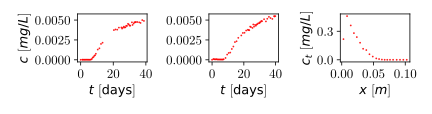
\includegraphics[width=\textwidth]{figs/core_data.pdf}
\footnotesize
Data from\\ \textit{``Entropy-based experimental design for optimal model discrimination in the geosciences''}\\ by \textcite{nowak2016entropy}
\end{frame}

%-------------------------------------------------------
\begin{frame}{Bayesian Neural Networks (BNNs)}
% Bayesian Neural Networks, or BNNs, treat the weights of a neural network as random variables.
% We start by assuming a prior distribution for these weights, which represents our initial beliefs about their values.
% Then, we use Bayes' theorem (point to the equation) to update these beliefs based on the observed data.
% This gives us a posterior distribution, which represents our updated knowledge about the weights after seeing the data.
% MCMC methods are a way to sample from this posterior distribution. They create a sequence of samples that, after an initial "burn-in" period, approximate the true posterior.
% So, in short, BNNs give us a way to quantify uncertainty in the parameters of a neural network by treating them as random variables and using Bayesian inference.
\centering

\only<1>{\includegraphics[width=0.8\textwidth]{figs/bnn_illustration.png}}

% \onslide<2>{
% \begin{tikzpicture}
% \node[opacity=0.3] at (0,0) {\includegraphics[width=0.8\textwidth]{figs/bnn_illustration.png}};
% \end{tikzpicture}
% }
% \vspace{-10pt}
\only<2->{

\begin{Large}
    \begin{equation*}
        \boxed{p(\theta | \mathcal{D}) \propto p(\mathcal{D} | \theta) p(\theta)}
    \end{equation*}
    \onslide<3->{
    \begin{equation*}
        \textcolor{red}{p(\hat{R}(c;\theta) | \mathcal{D})}
    \end{equation*}
    }
\end{Large}

\vfill % Push the table to the bottom


\begin{tabular}{rlrl} 
    $\theta$: & Weights and Biases & $p(\mathcal{D} | \theta)$: & Likelihood \\ 
    $\mathcal{D}$: & Training Data & $p(\theta | \mathcal{D})$: & Posterior \\
    $p(\theta)$: & Prior & \onslide<3->{$\hat{R}(c;\theta)$:} & \onslide<3->{Predicted Retardation Factor} \\
\end{tabular}

}
\end{frame}

%-------------------------------------------------------
\begin{frame}{Baseline (BNN with MCMC Sampling)}
% In the case we're considering here, we have a BNN that represents our retardation factor, R(c), and it has about 2000 parameters.
% So, when we use MCMC, we're essentially exploring a 2000-dimensional space, which is quite large.
% Even though 2000 parameters might seem like a lot, it's actually on the lower end for neural networks.
% Fortunately, we're still in a realm where these calculations are manageable, and we were able to obtain the following results (show image of MCMC samples).
% Here, we see the different datasets again - Core 1, Core 2, and Core 2B - and the corresponding FINN concentration predictions generated by the retardation factors sampled using MCMC, which are shown in the bottom right panel.
% In total, we generated 10,000 samples. As you can see, there's a nice variance in the sampled R(c) values, which reflects our uncertainty about the true retardation factor.
% In the following, I will now introduce our alternative method, and the BNN/MCMC method will serve as our baseline for comparison.
\centering
\includegraphics[width=0.95\textwidth]{figs/finn_mcmc_samples.pdf}

10,000 samples
% according to\\ \textit{``Learning groundwater contaminant diffusion-sorption processes with a finite volume neural network''}\\ by \textcite{finn}
\end{frame}

\section{Method}

%-------------------------------------------------------
\begin{frame}{NNPIE (Neural Network Prediction Interval Estimation)}
% Our method is based on the idea that we should treat all uncertainties in the problem as such, by representing them as random variables, similar to how BNNs do it.
% If we look at the FINN architecture again (show FINN architecture image), we can see that it's not just a simple mathematical formula.
% There are many design choices that go into it, and many of them are more or less uncertain in the sense that we don't know the "best" value.
% We decided to treat the following factors as uncertain: the initialization of the neural network parameters, the number of training epochs, the weighting between the MSE loss of the concentration data and the physical loss of FINN, and the training dataset itself.
% We distinguish between the hyperparameters, which are the first three, and the training dataset because they represent different types of uncertainty.
% If you'd like to know more about why we chose a specific parameter, feel free to ask me at the end.
% We'll now go through each of these factors one by one (show each parameter as a list item).
\centering
\only<1>{
\includegraphics[width=0.7\textwidth]{figs/finn_arch.png}
}

\only<2>{
\includegraphics[width=0.7\textwidth]{figs/loss_landscape.png}
}
\only<3->{
\begin{equation*}
    \mathcal{L} = \mathbf{a_{MSE}} \cdot Loss_{MSE} + \mathbf{a_{Phys}} \cdot Loss_{Phys}
\end{equation*}
}


\vfill

\begin{tabular}{rl}
    \textbf{Uncertain Factor} $\mathcal{X}$ & \textbf{Distribution} \\
    \hline
    Number of Epochs & Uniform(10, 30) \\
    \pause
    Weight Init. Seed & Discrete Uniform \\
    \pause
    $a_{MSE}$, \, $a_{Phys}$ & Log-Uniform($10^2$, $10^8$) \\
    \pause
    Training Dataset & $p(\mathcal{D})$
\end{tabular}
% We call the first method 'Hyperparameter Neural Network Prediction Interval Estimation', or Hy-NNPIE for short.
\end{frame}

%-------------------------------------------------------
\begin{frame}{Hy-NNPIE - Samples}
% For this, we sampled 780 hyperparameter vectors from the distributions listed here (show table with distributions).
% For each vector, we trained FINN on the BTC-2 dataset and obtained these output samples (show image with Hy-NNPIE samples).
% We get a similar picture as with the baseline. However, these samples are not yet drawn from the correct distribution.
% What we've done so far is roughly equivalent to a sensitivity analysis of FINN with respect to the hyperparameters.
\centering
\includegraphics[width=0.95\textwidth]{figs/finn_span_samples.pdf}
780 samples
\end{frame}

%-------------------------------------------------------
\begin{frame}{NNPIE - Distribution Derivation}
% A bit of math tells us how we need to weight the samples to draw from the same distribution as the baseline (show derivation of p(R|D)).
% The weights require the same likelihood that the baseline also needed, so we use the same one, which corresponds to a Gaussian distribution around the training data.
\begin{align*}
\onslide<1->{p(\hat{R}(c;\theta_{\mathcal{X}}) = R(c)| &\mathcal{D})} \\
\onslide<2->{\small{\text{(Marginalization)}} \quad &= \int p(\hat{R}(c;\theta_{\mathcal{X}}) = R(c) | \mathcal{X}, \mathcal{D})\; p(\mathcal{X} | \mathcal{D}) \, d\mathcal{X}} \\
                                         \onslide<3->{\small{\text{(Bayes)}} \quad &= \int p(\hat{R}(c;\theta_{\mathcal{X}}) = R(c) | \mathcal{X}, \mathcal{D})\; p(\mathcal{X}) \underbrace{\frac{p(\mathcal{D} | \mathcal{X}) }{p(\mathcal{D})}}_{= w(\mathcal{X})} \, d\mathcal{X} \\
                                          &= \int p(\hat{R}(c;\theta_{\mathcal{X}}) = R(c) | \mathcal{X}, \mathcal{D})\; p(\mathcal{X})\; w(\mathcal{X}) \, d\mathcal{X}} \\
                                         \onslide<4->{\small{\text{(Determ. Solver)}} \quad &= \int \delta(\hat{R}(c;\theta_{\mathcal{X}}) - R(c))\; p(\mathcal{X})\; w(\mathcal{X}) \, d\mathcal{X} .}
\end{align*}
\end{frame}

%-------------------------------------------------------
\begin{frame}{Hy-NNPIE vs. MCMC (90\% PIs)}
% Finally, we get a distribution from which we can now plot the 90% prediction interval, or PI (show image of MCMC vs. Hy-NNPIE).
% We can see that our method predicts a significantly narrower PI for the retardation factor.
% However, the PI around the concentration is also much smaller, which still gives us some leeway.
\centering
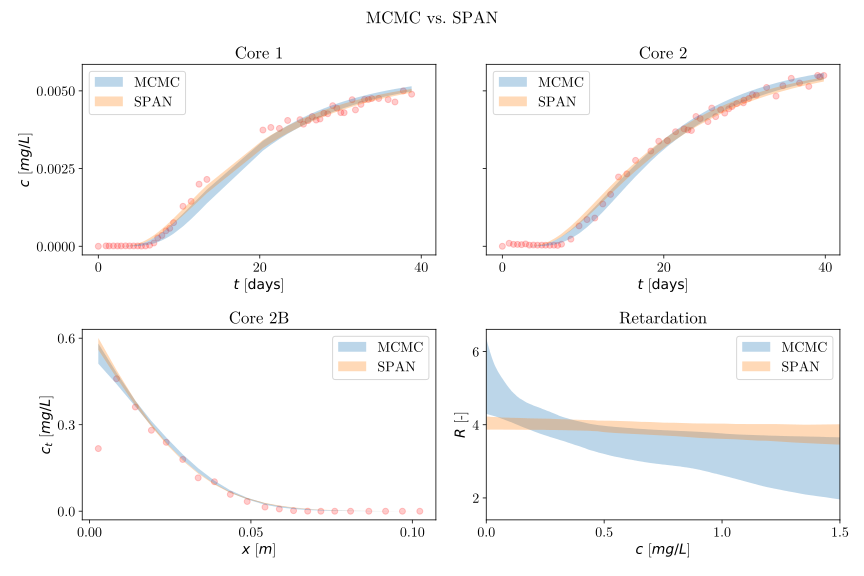
\includegraphics[height=0.9\textheight]{figs/finn_MCMCvsSPAN_PIs.pdf}
\end{frame}

%-------------------------------------------------------
\begin{frame}{Da-NNPIE}
% The last uncertainty we considered was the dataset itself, also known as aleatoric uncertainty.
% Here, it's not as straightforward to determine how to choose the dataset samples, that is, the distribution of the dataset.
% We first tried two different methods on a synthetic dataset, one without noise (show image of full c field).
% This synthetic dataset, in contrast to the experimental one, consists of concentration data over space and time, so it contains much more data.
% It was generated using retardation factors defined by a known parametric isotherm. Here, we used the Langmuir isotherm (show image of parametric isotherms).
\centering
\includegraphics[width=0.8\textwidth]{figs/c_diss_field_full.pdf}
\pause
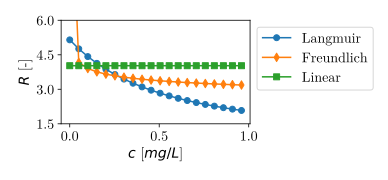
\includegraphics[width=0.6\textwidth]{figs/parametric_isotherms.pdf}
\end{frame}

%-------------------------------------------------------
\begin{frame}{Da-NNPIE - Variant 1: Masked Dataset}
% The first dataset sampling method is known as data subsetting.
% Here, values are randomly removed from the dataset, and the model is trained only on a subset.
% We removed 50% of the synthetic data points (show image with loss patterns).
% (Show result image and hide the previous one.)
\centering
\only<1>{\includegraphics[width=0.9\textwidth]{figs/c_diss_field_train_random_subset.pdf}}
\only<2>{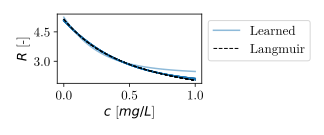
\includegraphics[width=0.7\textwidth]{figs/finn_synthetic_SPAN_losspattern.pdf}}
\end{frame}

%-------------------------------------------------------
\begin{frame}{Da-NNPIE - Variant 2: Gaussian Noise}
% In the second method, we wanted to mimic the experimental case and added Gaussian noise of the same magnitude as in the experiment to the data
\centering
\only<1>{\includegraphics[width=0.9\textwidth]{figs/c_diss_field_plus_noise.pdf}}
\only<2>{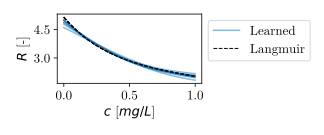
\includegraphics[width=0.7\textwidth]{figs/finn_synthetic_SPAN_noise.pdf}}
\only<3>{
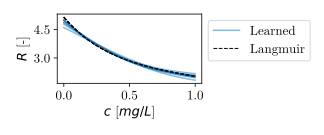
\includegraphics[width=0.4\textwidth]{figs/finn_synthetic_SPAN_noise.pdf}
\includegraphics[width=0.4\textwidth]{figs/MCMC_ret_samples.png}
}
\end{frame}

%-------------------------------------------------------
\begin{frame}{Da-NNPIE - Variant 3: PI3NN Method}
% Both of these methods were not as successful as the first one (Hy-NNPIE).
% This is because neural networks with an MSE loss learn the mean, which hardly changes for the dataset samples generated by these two methods.
% So, we developed a new method where we generate dataset samples that have different means.
% For this, we use PI3NN.
% PI3NN is a method for constructing prediction intervals using three independently trained neural networks.
% It approximates the median of the target variable and the expected deviations above and below the median.
% Once trained, PI3NN constructs the PI bounds as linear combinations of the three networks' outputs.
% The coefficients of these linear combinations are determined through a root-finding algorithm that ensures the desired coverage probability for a given confidence level.
\centering
\includegraphics[width=0.95\textwidth]{figs/3pinn_illustration_talk.pdf}
\end{frame}

%-------------------------------------------------------
\begin{frame}{Da-NNPIE - PI3NN-based Sampling}
% Applied to our BTC-2, we generated 70 samples (show image with PI3NN BTC-2 dataset) ...
\centering
\includegraphics[height=0.9\textheight]{figs/btc_dataspan_quantiles_talk.pdf}
\end{frame}

%-------------------------------------------------------
\begin{frame}{Da-NNPIE - Samples}
% ... and used them to learn the following retardation factors (show image with Da-NNPIE samples).
% Again, we need to correct the samples with weights, and we obtain ...
\centering
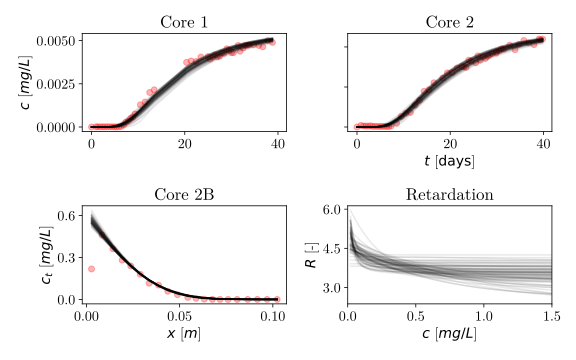
\includegraphics[width=0.95\textwidth]{figs/finn_dataspan_samples.pdf}

70 samples
\end{frame}

%-------------------------------------------------------
\begin{frame}{Da-NNPIE vs. MCMC (90\% PIs)}
% ... the following 90% prediction intervals (show image of MCMC vs. Da-NNPIE).
% We can see that we are qualitatively much closer here.
\centering
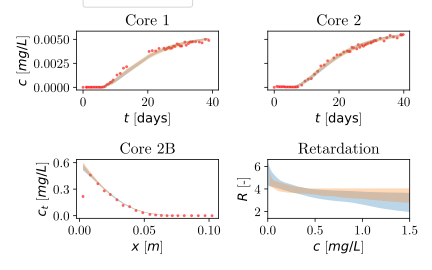
\includegraphics[height=0.9\textheight]{figs/finn_MCMCvsData-SPAN_PIs.pdf}
\end{frame}

%-------------------------------------------------------
\begin{frame}{HyDa-NNPIE vs. MCMC (90\% PIs)}
% Of course, 'Hy-NNPIE' and 'Da-NNPIE' can also be combined, but the difference to pure Da-NNPIE was negligible (show image of HyDa-NNPIE vs. MCMC).
\centering
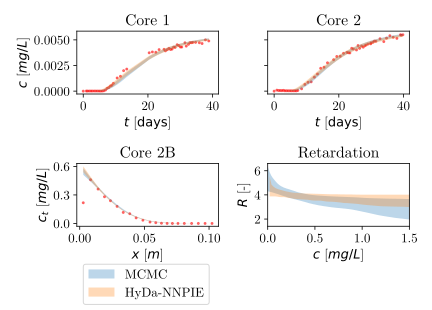
\includegraphics[height=0.9\textheight]{figs/finn_MCMCvsFull-SPAN_PIs.pdf}
\end{frame}

\section{Quantitative Evaluation}

%-------------------------------------------------------
\begin{frame}{Likelihood Comparison}
    % Even though we now have PIs for R(c), it's still unclear whether our method is better than the baseline.
    % Our R(c) PI is a bit narrower, and the concentration PIs are roughly the same.
    % We can use the concentration samples together with the dataset to calculate the likelihood (explain how we quantitatively evaluate the methods).
    \centering
    \only<1>{\includegraphics[width=0.95\textwidth]{figs/likelihood_explanation_0.pdf}}
    \only<2>{\includegraphics[width=0.95\textwidth]{figs/likelihood_explanation_1.pdf}}
    \only<3>{\includegraphics[width=0.95\textwidth]{figs/likelihood_explanation_2.pdf}}
    \only<4>{\includegraphics[width=0.95\textwidth]{figs/likelihood_explanation_3.pdf}}
    \only<5>{\includegraphics[width=0.95\textwidth]{figs/likelihood_explanation_4.pdf}}
    \only<6,8>{\includegraphics[width=0.95\textwidth]{figs/nll_comparison.pdf}}
    \only<7>{
    Gaussian Fit with sample standard deviation computed from the residuals:
    \vfill
    \includegraphics[width=0.6\textwidth]{figs/c_gauss_fit.png}
    }
\end{frame}


%-------------------------------------------------------
\begin{frame}{Runtime Comparison}
    \centering
    \includegraphics[width=0.9\textwidth]{figs/runtime_comparison.pdf}
    \begin{itemize}
        \item NNPIE: 70 samples
        \item MCMC: 10,000 samples
    \end{itemize}
\end{frame}


%-------------------------------------------------------
\begin{frame}{Conclusion}
    \centering
    \textbf{NNPIE Advantages:}
    \begin{itemize}
        \pause
        \item[*] PIs of comparable Quality
        \pause
        \item[*] Faster Computation
        \item[*] Easier Parallelization
    \end{itemize}
    \pause
    \vfill
    \Large{
    Thank you for your attention.
    }
\end{frame}


%-------------------------------------------------------




% There are two possible final slide layouts (white and blue). Choose one of them!
% You need five arguments:
% 1) Text phrase ("Thank you!"), 2) Your Name, 3) E-Mail-Address 4) Phonenumber of whatever you want (or leave empty)
% 5) An image for the cicle on the left (for example Logo of the institute)
% \thankyou{Thank you for your attention!}{Riccardo Frenner}{st161374@stud.uni-stuttgart.de}{}{gfx/abschluss.jpg}
\thankyoublue{Thank you!}{Riccardo Frenner}{st161374@stud.uni-stuttgart.de}{}{gfx/logos/ls3_logo_white_bg.png}

\begin{frame}{References}
\printbibliography
\end{frame}


% Appendix
\begin{frame}{PI Calibration Comparison}
    % (Explain calibration and show image of reliability curves.)
    \centering
    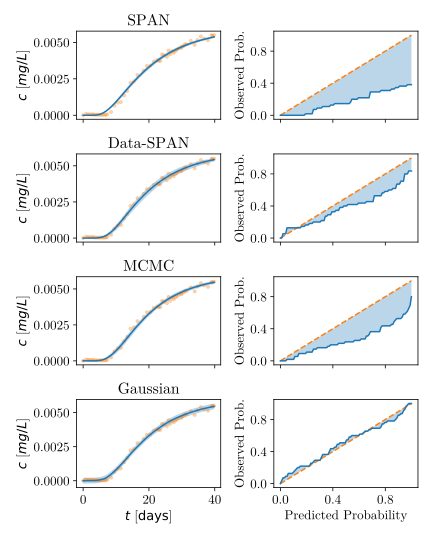
\includegraphics[height=0.9\textheight]{figs/reliability_curves.pdf}
\end{frame}


\end{document}
